\documentclass[a4paper,12pt,scale=0.8][UTF8]{ctexart}
\usepackage[margin=2in]{geometry} % 設定邊界
\usepackage[usenames]{color} %pour la couleur
\usepackage{ctex}
\usepackage{amssymb} %maths
\usepackage{amsmath} %maths
\usepackage{hyperref}
\begin{document}
~~~~~~~~~~~~~~~\textbf{2019-2020学年第二学期八年级数学教学质量检测} \\
 \\
 \\
 \\
\textbf{一、选择题}:\textbf{本题共10小题},\textbf{每小题4分},\textbf{共40分.在每小题给出的四个选项中},\textbf{只有一项是符合题目要求的.} \\
 \\
1{[}单选题{]}
函数\(y = \mathrm{\lg}\frac{x}{x - 2} + \mathrm{\arcsin}\frac{x}{3}\)
的定义域是( )。\\
{[}选项{]}{[}纵向平铺{]} \\ % 选项关键字及选项展示格式 横向平铺,纵向平铺,网格。
A. \(\left\lbrack - 3,\ \ 0 \right) \cup (2,\ 3\rbrack\)

B. \(\lbrack - 3,\ 3\rbrack\)

C. \(\left\lbrack - 3,\ 0 \right)\  \cup \ \ (1,\ 3\rbrack\)

D. \(\left\lbrack - 2,\ 0 \right) \cup (1,\ 2)\)

{[}答案{]}A \\
{[}分数{]}4 \\
{[}学科{]}数学 \\
{[}难度{]}容易 \\  % 难度有容易、中档、困难
{[}解析{]} \\
2{[}单选题{]}如图,在矩形\emph{ABCD}中,\emph{AB}\textless{}\emph{BC},\emph{AC},\emph{BD}相交于点\emph{O},则图中等腰三角形的个数是( ) \\
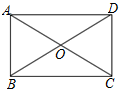
\includegraphics[width=1.24984in,height=0.9478in]{/Users/hepengfei/data/goproject/src/yokitalk.com/docservice/template/image/media/image2.png} \\

{[}选项{]}{[}横向平铺{]} \\ % 选项关键字及选项展示格式 横向平铺,纵向平铺,网格。
A.\(8\)~~B.\(6\)~~C.\(4\)~~D.\(2\)

{[}答案{]}C \\
{[}分数{]}4 \\
{[}学科{]}数学 \\
{[}难度{]}容易 \\  % 难度有容易、中档、困难
{[}解析{]} \\
3{[}单选题{]}下列四对\emph{x},\emph{y}的值是二元一次方程3\emph{x}+\emph{y}=5的解的是( )

{[}选项{]}{[}横向平铺{]} \\ % 选项关键字及选项展示格式 横向平铺,纵向平铺,网格。
A. B. C. D.

{[}答案{]}B \\
{[}分数{]}4 \\
{[}学科{]}数学 \\
{[}难度{]}容易 \\  % 难度有容易、中档、困难
{[}解析{]} \\
4{[}单选题{]}如图,\emph{O}为直线\emph{AB}上一点,\emph{OE}平分∠\emph{BOC},\emph{OD}⊥\emph{OE}于点\emph{O},若∠\emph{BOC}=80°,则∠\emph{AOD}的度数是( )

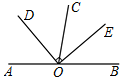
\includegraphics[width=1.29097in,height=0.83264in]{/Users/hepengfei/data/goproject/src/yokitalk.com/docservice/template/image/media/image9.png}

{[}选项{]}{[}网格{]} \\ % 选项关键字及选项展示格式 横向平铺,纵向平铺,网格。

A.70° B.50°

C.40° D.35°

{[}答案{]}B \\
{[}分数{]}4 \\
{[}学科{]}数学 \\
{[}难度{]}中档 \\  % 难度有容易、中档、困难
{[}解析{]} \\
\end{document}
